\documentclass[12pt,a4paper]{article}

% ── Packages ──────────────────────────────────────────────────────────────────
\usepackage[top=1in, bottom=1in, left=0.7in, right=0.7in]{geometry}
\usepackage{graphicx}
\usepackage{amsmath,amssymb}
\usepackage{booktabs}
\usepackage{tabularx}
\usepackage{xcolor}
\usepackage{hyperref}
\usepackage{algorithm}
\usepackage{algpseudocode}
\usepackage{tikz}
\usepackage{tikz-layers}
\usetikzlibrary{shapes.geometric, arrows.meta, positioning, fit, backgrounds,
                decorations.pathreplacing, calc}
\usepackage{float}
\usepackage{caption}
\usepackage{subcaption}
\usepackage{listings}
\usepackage{enumitem}
\usepackage{fancyhdr}
\usepackage{titlesec}
\usepackage{parskip}
\usepackage{mdframed}
\usepackage{tcolorbox}
\tcbuselibrary{skins,breakable}
\usepackage{multirow}
\usepackage{array}
\usepackage{cite}
\usepackage{url}

% ── Colours ───────────────────────────────────────────────────────────────────
\definecolor{iitgblue}{RGB}{0,56,101}
\definecolor{accentblue}{RGB}{30,100,200}
\definecolor{lightgray}{RGB}{245,245,245}
\definecolor{darkgray}{RGB}{80,80,80}
\definecolor{codegreen}{RGB}{0,128,0}
\definecolor{codepurple}{RGB}{128,0,128}
\definecolor{contrib}{RGB}{220,240,255}
\definecolor{contribborder}{RGB}{30,100,200}
\definecolor{noteboxbg}{RGB}{255,250,230}
\definecolor{noteboxborder}{RGB}{200,150,0}

% ── Hyperref setup ─────────────────────────────────────────────────────────────
\hypersetup{
  colorlinks=true,
  linkcolor=accentblue,
  citecolor=iitgblue,
  urlcolor=accentblue,
  pdftitle={CS525 Project Report -- Group 2},
  pdfauthor={Pranjal, Dhruv R Pansuriya, Shrish Uttarwar}
}

% ── Listings (code) ────────────────────────────────────────────────────────────
\lstset{
  backgroundcolor=\color{lightgray},
  basicstyle=\ttfamily\small,
  keywordstyle=\color{accentblue}\bfseries,
  commentstyle=\color{codegreen}\itshape,
  stringstyle=\color{codepurple},
  frame=single,
  rulecolor=\color{darkgray},
  breaklines=true,
  numbers=left,
  numberstyle=\tiny\color{darkgray},
  xleftmargin=1em,
  framexleftmargin=1.5em,
  captionpos=b
}

% ── Section formatting ─────────────────────────────────────────────────────────
\titleformat{\section}{\large\bfseries\color{iitgblue}}{{\thesection.}}{0.6em}{}[\titlerule]
\titleformat{\subsection}{\normalsize\bfseries\color{accentblue}}{{\thesubsection}}{0.5em}{}
\titleformat{\subsubsection}{\normalsize\bfseries\color{black}}{{\thesubsubsection}}{0.4em}{}

% ── Header / Footer ───────────────────────────────────────────────────────────
\pagestyle{fancy}
\fancyhf{}
\fancyhead[L]{\small\color{darkgray}CS525 -- Formal Methods for System Verification}
\fancyhead[R]{\small\color{darkgray}Group 2 $\mid$ Project 2 $\mid$ Final Report}
\fancyfoot[C]{\small\thepage}
\renewcommand{\headrulewidth}{0.4pt}

% ── TikZ styles ───────────────────────────────────────────────────────────────
\tikzset{
  block/.style={rectangle, draw=iitgblue, fill=contrib, rounded corners=4pt,
                text width=4.6cm, align=center, minimum height=1cm,
                font=\small\bfseries},
  block2/.style={rectangle, draw=accentblue, fill=noteboxbg, rounded corners=4pt,
                text width=3.8cm, align=center, minimum height=0.9cm,
                font=\small},
  smallbox/.style={rectangle, draw=darkgray, fill=white, rounded corners=3pt,
                text width=2.8cm, align=center, minimum height=0.8cm,
                font=\scriptsize},
  arrow/.style={-Stealth, thick, color=iitgblue},
  dasharrow/.style={-Stealth, dashed, thick, color=darkgray},
  groupbox/.style={draw=darkgray, dashed, rounded corners=6pt,
                   fill=gray!5, inner sep=8pt}
}

% ── Contribution box ──────────────────────────────────────────────────────────
\newenvironment{contribbox}[1]{%
  \begin{tcolorbox}[
    colback=contrib,
    colframe=contribborder,
    title={\bfseries\color{iitgblue} #1},
    fonttitle=\small,
    breakable,
    left=6pt, right=6pt, top=4pt, bottom=4pt
  ]
}{%
  \end{tcolorbox}
}

\newenvironment{notebox}[1]{%
  \begin{tcolorbox}[
    colback=noteboxbg,
    colframe=noteboxborder,
    title={\bfseries\color{darkgray} #1},
    fonttitle=\small,
    breakable,
    left=6pt, right=6pt, top=4pt, bottom=4pt
  ]
}{%
  \end{tcolorbox}
}

% ══════════════════════════════════════════════════════════════════════════════
\begin{document}
% ══════════════════════════════════════════════════════════════════════════════

% ── Title Page ────────────────────────────────────────────────────────────────
\begin{titlepage}
  \centering
  \vspace*{0.4cm}

  % Institution heading
  {\color{iitgblue}\rule{\linewidth}{2pt}}
  \vspace{0.3cm}

  {\Large\bfseries\color{iitgblue}
    CS525 -- Formal Methods for System Verification}\\[0.2cm]
  {\normalsize Course Project -- Final Report}

  \vspace{0.4cm}
  {\color{iitgblue}\rule{\linewidth}{0.2pt}}
  \vspace{0.6cm}

  % Title
  {\LARGE\bfseries\color{iitgblue}
    LLM-Driven SystemVerilog Assertion Generation\\[0.2cm]
    for Formal Verification}

  \vspace{0.4cm}
  {\large\color{darkgray}\itshape
    Addressing Long-Context Understanding, Efficient Communication,\\
    and Structured Reasoning for Scalable Assertion Synthesis}

  \vspace{1.2cm}

  % Group info
    {\bfseries\color{iitgblue} Group 2 $\;\cdot\;$ Project 2}\\[6pt]
    \begin{tabular}{lc}
      \bfseries Pranjal           & \texttt{230101077} \\[2pt]
      \bfseries Dhruv R Pansuriya & \texttt{230101071} \\[2pt]
      \bfseries Shrish Uttarwar   & \texttt{230101108} \\
    \end{tabular}

  \vspace{4.0cm}

  {\normalsize\color{darkgray}
    \textbf{Date:} 25 April 2026}
    
  \vspace{0.4cm}
  {\color{iitgblue}\rule{\linewidth}{0.8pt}}
  \vspace{0.6cm}

  {\Large\bfseries\color{iitgblue}
    Indian Institute of Technology Guwahati}\\[0.2cm]
  {\normalsize Department of Computer Science \& Engineering}

\end{titlepage}

% ══════════════════════════════════════════════════════════════════════════════
\section{Abstract}
% ══════════════════════════════════════════════════════════════════════════════

Formal Verification (FV) is a cornerstone of reliable hardware design, and
SystemVerilog Assertions (SVAs) are the primary mechanism through which
design correctness is specified and validated. However, writing high-quality
assertions remains a challenging, expert-driven, and error-prone task.
Recent Large Language Model (LLM)-based approaches aim to automate SVA
generation, but face significant limitations including restricted context
windows, fragmented design understanding, and inefficiencies in multi-step
reasoning.

In this report, we present our final system for \textbf{LLM-driven SVA
generation}, developed as part of \textbf{Project~2} in \textbf{CS525}. Our
approach is inspired by recent structured pipelines for assertion synthesis,
but extends them with a focus on addressing five core challenges: 
\textit{(i) long-context limits, (ii) agent memory, (iii) cloud communication
efficiency, (iv) redundancy in multi-agent systems, and (v) feedback-driven
refinement}. 

We design a modular pipeline that integrates structured representations
of specifications and RTL, retrieval-driven context selection, prompt
compression, and iterative refinement mechanisms. Our system incorporates
techniques such as knowledge structuring, memory augmentation, and efficient
prompting strategies to improve both the quality and scalability of generated
assertions. 

Through this work, we demonstrate how LLM-based assertion generation can be
made more context-aware, cost-efficient, and robust, moving closer to practical
deployment in real-world formal verification workflows.
% ══════════════════════════════════════════════════════════════════════════════
\section{Introduction}
% ══════════════════════════════════════════════════════════════════════════════

Assertion-Based Verification (ABV) is the dominant paradigm for ensuring that
VLSI designs behave according to specification. SVAs allow engineers to express
properties such as \textit{``whenever a request is asserted, an acknowledgement
must follow within three clock cycles''}, which formal tools can exhaustively
verify. The primary bottleneck, however, is that writing SVAs requires
simultaneously understanding high-level specification documents (often
hundreds of pages of natural language) and low-level RTL implementations
(thousands of lines of code).

Existing LLM-based methods such as AssertLLM~\cite{assertllm} rely heavily on
either specification text or RTL in isolation. This leads to incomplete design
understanding: specification-only approaches miss implementation-level details,
while RTL-only approaches lack the intended behavior captured in natural
language. Consequently, generated assertions are often syntactically correct
but semantically inaccurate.

Recent structured approaches attempt to bridge this gap by decomposing the
problem into intermediate representations and multi-stage pipelines. Building
on these ideas, our work focuses on addressing a key systems challenge:

\begin{center}
\textit{How can an automated system synthesise information from ambiguous,
multi-page natural-language specifications and complex RTL code to generate
SVAs that are both syntactically correct and functionally meaningful — within
the token and cost constraints of modern LLMs?}
\end{center}

Our project addresses this challenge through five specific sub-problems:

\begin{enumerate}[leftmargin=*, label=\textbf{P\arabic*.}]
  \item \textbf{Long-Context Limits} --- selecting a minimal, sufficient context subset.
  \item \textbf{Agent Memory} --- accumulating and reusing verified knowledge across steps.
  \item \textbf{Cloud Communication Efficiency} --- reducing API token and latency overhead.
  \item \textbf{Redundancy in Multi-Agent Systems} --- minimizing duplicated computation and assertions.
  \item \textbf{Feedback-Driven Refinement} --- improving outputs using verifier or critic feedback.
\end{enumerate}

\noindent
This report presents our final system design, implementation, and evaluation,
demonstrating how these challenges can be jointly addressed in a unified
LLM-driven verification pipeline.
% ══════════════════════════════════════════════════════════════════════════════
\section{Related Work}
% ══════════════════════════════════════════════════════════════════════════════

\subsection{AssertLLM}

AssertLLM~\cite{assertllm} is one of the earliest end-to-end pipelines for
automating SVA generation from natural-language specifications. It decomposes
the task into three stages: structural specification extraction, signal
mapping, and assertion synthesis. This staged design highlights the importance
of intermediate representations when bridging natural language and RTL-level
semantics.

However, a key limitation of AssertLLM is that it operates primarily on
specification documents, without incorporating sufficient information from
the RTL implementation. As a result, when specifications are ambiguous or
incomplete, the generated assertions may appear plausible but fail under
formal verification. This limitation motivates the need for approaches that
jointly reason over both specification intent and implementation details.

\begin{figure}[h]
    \centering
    \includegraphics[width=0.8\linewidth]{assert_llm.png}
    \caption{AssertLLM in VLSI design and verification flow. The system
automatically generates SVAs from natural language specifications,
supporting functional verification and bug detection.}
    \label{fig:assertllm}
\end{figure}

\subsubsection{Challenges in Understanding and Implementation}

Despite its conceptual clarity, reproducing or extending AssertLLM presents
several practical challenges:

\begin{itemize}
    \item \textbf{Ambiguity in natural language specifications:} Translating
    informal and underspecified requirements into precise formal properties
    remains inherently difficult.

    \item \textbf{Limited implementation transparency:} The original work
    provides only a high-level pipeline description, with minimal details on
    prompt design, intermediate representations, model configurations, and
    post-processing. Critical steps such as structural extraction, signal
    alignment, and ambiguity resolution are not concretely specified, making
    faithful reproduction challenging.
\end{itemize}

\subsection{ClarifyGPT --- Insufficiency Detection}

ClarifyGPT~\cite{clarifygpt} addresses ambiguity in user requirements by
detecting inconsistencies across multiple generated outputs. The system
generates alternative solutions and evaluates whether they produce consistent
results; discrepancies indicate insufficient or ambiguous input. It then
generates targeted clarification questions to resolve these gaps.

This idea is directly relevant to SVA generation, where incomplete context can
lead to incorrect assertions. Instead of producing potentially invalid SVAs,
a system should detect when available information is insufficient and trigger
clarification or additional context retrieval. While ClarifyGPT operates in a
code-generation setting, its core principle of \emph{insufficiency detection}
informs our approach to robust assertion synthesis.

\subsection{STELLAR --- Structure-Guided SVA Retrieval}

STELLAR (2025) proposes a structure-aware retrieval mechanism for improving
SVA generation. Rather than relying solely on semantic similarity, it encodes
RTL blocks using Abstract Syntax Tree (AST) structural features and retrieves
similar (RTL, SVA) pairs from a knowledge base. These examples are then used
as few-shot prompts for the LLM.

The key insight is that structurally similar RTL patterns often correspond to
similar assertion templates. By leveraging structural fingerprints instead of
pure textual similarity, STELLAR improves retrieval relevance and generation
quality. This highlights the importance of incorporating structural program
information into LLM-based verification pipelines.

% ══════════════════════════════════════════════════════════════════════════════
\section{Algorithm Deep Dive}
% ══════════════════════════════════════════════════════════════════════════════

AssertionForge~\cite{assertionforge} is a two-stage, three-component pipeline.
We studied the paper and source code in detail. Figure~\ref{fig:pipeline}
illustrates the complete workflow.

\begin{figure}[H]
\centering
\resizebox{\linewidth}{!}{%
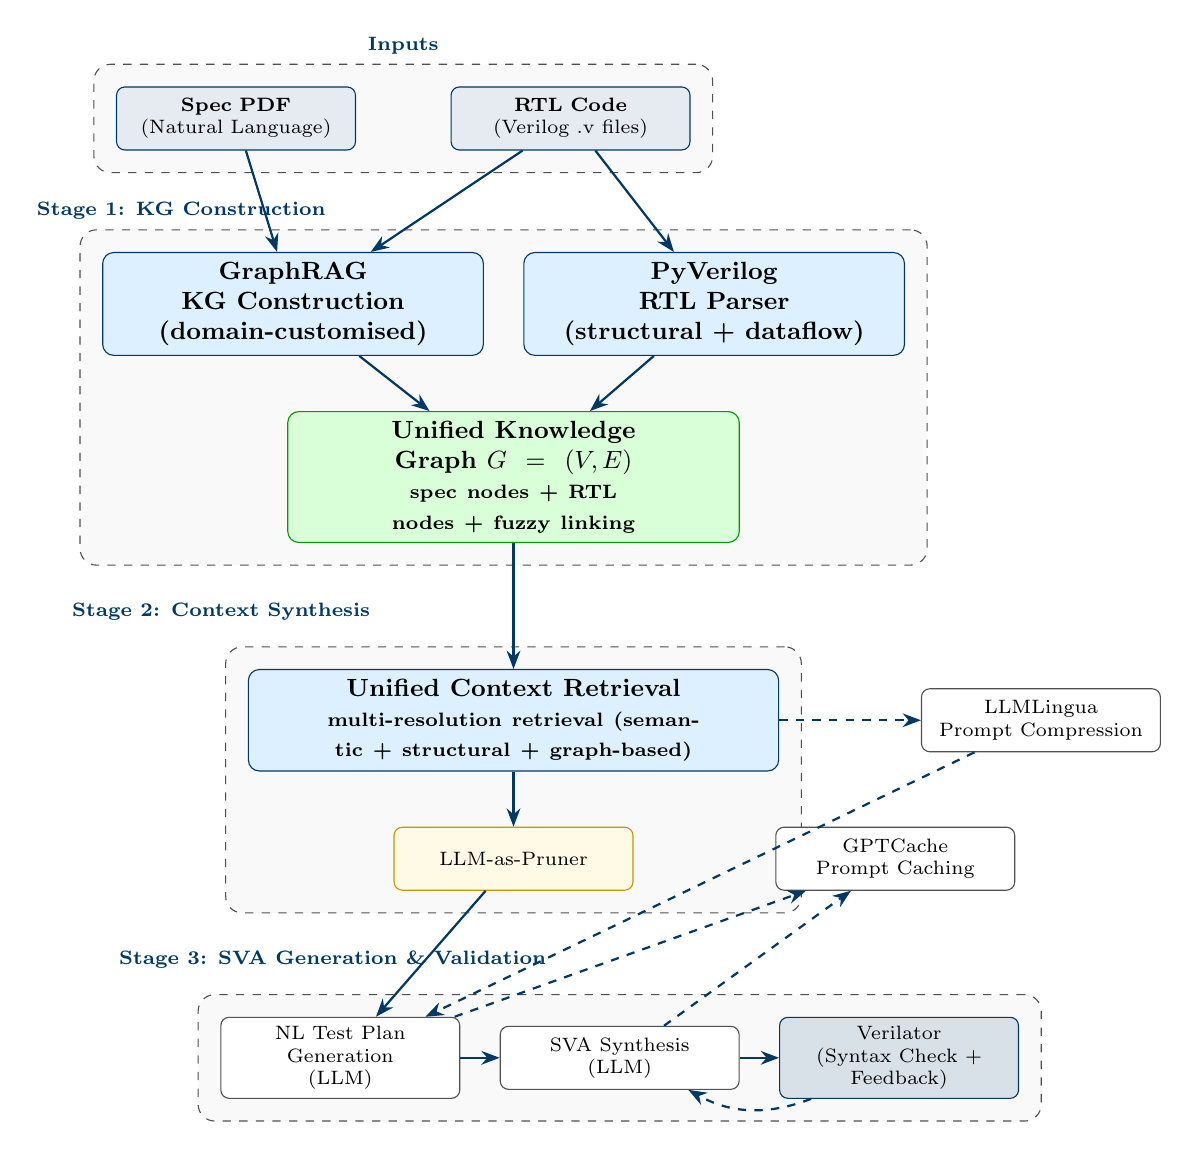
\begin{tikzpicture}[node distance=0.7cm and 0.5cm]

  %% ── Inputs ────────────────────────────────────────────────────────────
  \node[smallbox, fill=iitgblue!10, draw=iitgblue] (spec)
        {\textbf{Spec PDF}\\(Natural Language)};
  \node[smallbox, fill=iitgblue!10, draw=iitgblue, right=1.2cm of spec] (rtl)
        {\textbf{RTL Code}\\(Verilog .v files)};

  \begin{scope}[on background layer]
    \node[groupbox, fit=(spec)(rtl), label={[font=\scriptsize\bfseries, color=iitgblue]above:Inputs}] (inputgrp) {};
  \end{scope}

  %% ── Stage 1: KG ────────────────────────────────────────────────────────
  \node[block, below=1.0cm of inputgrp, xshift=-1.4cm] (graphrag)
        {GraphRAG\\KG Construction\\(domain-customised)};
  \node[block, right=0.5cm of graphrag] (rtlparse)
        {PyVerilog\\RTL Parser\\(structural + dataflow)};

  \node[block, fill=green!15, draw=green!60!black, below=0.7cm of graphrag,
        xshift=2.8cm, text width=5.5cm] (kg)
        {\textbf{Unified Knowledge Graph $G=(V,E)$}\\
         \scriptsize spec nodes + RTL nodes + fuzzy linking};

  \begin{scope}[on background layer]
    \node[groupbox, fit=(graphrag)(rtlparse)(kg),
          label={[font=\scriptsize\bfseries, color=iitgblue]above left:Stage 1: KG Construction}] (stage1) {};
  \end{scope}

  %% ── Stage 2: Context ────────────────────────────────────────────────────
  \node[block, below=1.6cm of kg, text width=6.5cm, align=center] (context)
        {\textbf{Unified Context Retrieval}\\
         \scriptsize multi-resolution retrieval (semantic + structural + graph-based)};

  \node[smallbox, fill=noteboxbg, draw=noteboxborder,
        below=0.7cm of context] (pruner)
        {LLM-as-Pruner};

  \begin{scope}[on background layer]
    \node[groupbox, fit=(context)(pruner),
          label={[font=\scriptsize\bfseries, color=iitgblue, yshift=0.2cm]above left:Stage 2: Context Synthesis}] (stage2) {};
  \end{scope}

  %% ── Auxiliary Components ────────────────────────────────────────────────
  \node[smallbox, right=1.8cm of context] (lingua)
        {LLMLingua\\Prompt Compression};

  \node[smallbox, right=1.8cm of pruner] (cache)
        {GPTCache\\Prompt Caching};

  %% ── Stage 3: Generation ─────────────────────────────────────────────────
  \node[smallbox, below=1.6cm of pruner, xshift=-2.2cm] (nlplan)
        {NL Test Plan\\Generation\\(LLM)};
  \node[smallbox, right=0.5cm of nlplan] (svasynth)
        {SVA Synthesis\\(LLM)};
  \node[smallbox, fill=iitgblue!15, draw=iitgblue,
        right=0.5cm of svasynth] (verilator)
        {Verilator\\(Syntax Check +\\Feedback)};

  \begin{scope}[on background layer]
    \node[groupbox, fit=(nlplan)(svasynth)(verilator),
          label={[font=\scriptsize\bfseries, color=iitgblue, yshift=0.2cm]above left:Stage 3: SVA Generation \& Validation}] (stage3) {};
  \end{scope}

  %% ── Arrows ──────────────────────────────────────────────────────────────
  \draw[arrow] (spec) -- (graphrag);
  \draw[arrow] (rtl)  -- (rtlparse);
  \draw[arrow] (rtl)  -- (graphrag);

  \draw[arrow] (graphrag) -- (kg);
  \draw[arrow] (rtlparse) -- (kg);

  \draw[arrow] (kg) -- (context);
  \draw[arrow] (context) -- (pruner);

  \draw[arrow] (pruner) -- (nlplan);
  \draw[arrow] (nlplan) -- (svasynth);
  \draw[arrow] (svasynth) -- (verilator);

  %% Feedback loop
  \draw[arrow, dashed] (verilator) to[bend left=25] (svasynth);

  %% Optional connections (light/dashed to show auxiliary role)
  \draw[arrow, dashed] (context) -- (lingua);
  \draw[arrow, dashed] (lingua) -- (nlplan);

  \draw[arrow, dashed] (nlplan) -- (cache);
  \draw[arrow, dashed] (svasynth) -- (cache);

\end{tikzpicture}
}
\caption{End-to-end LLM-driven SVA generation pipeline. The system integrates structured knowledge extraction, unified context retrieval, prompt optimization (LLMLingua), caching (GPTCache), and syntax-driven feedback (Verilator) for iterative refinement.}
\label{fig:pipeline}
\end{figure}

\subsection{Stage 1: Knowledge Graph Construction}

\subsubsection{Specification-Side: GraphRAG with Domain-Customised Schema}

AssertionForge begins by constructing an initial KG $G_0$ from the
specification document. It leverages Microsoft GraphRAG~\cite{graphrag}, a
framework that (i) chunks source text, (ii) uses an LLM to extract entities
and relationships, (iii) summarises node/edge descriptions, and (iv) assembles
a graph. The critical novelty is that AssertionForge replaces GraphRAG's
generic entity-extraction prompt with a hardware-specific schema $\Sigma =
(E_t, R_t)$:

\begin{itemize}[noitemsep]
  \item \textbf{Entity types $E_t$:} Design Specification, Module, Submodule,
        Signal, Port, Register, FIFO, Clock, Interrupt, Protocol, Operation,
        Constraint/Rule, Address, FSM.
  \item \textbf{Relation types $R_t$:} \texttt{connectsTo}, \texttt{defines},
        \texttt{triggers}, \texttt{dependsOn}, \texttt{generatesInterrupt},
        \texttt{operatesAt}, \texttt{transmitsData}, \texttt{HasSignal},
        \texttt{UsesClock}, \texttt{DescribesOperation}, \textit{etc.}
\end{itemize}

Node attributes include entity type, description, source chunk ID, degree, and
level. Edge attributes include weight and description. The schema is discovered
semi-automatically: a small set of specification excerpts is shown to the LLM,
which proposes entity/relation types; a human expert then merges redundant
concepts (e.g., ``Reset Signal'' and ``Reset'').

\subsubsection{RTL-Side: PyVerilog Parser and KG Refinement}

The initial $G_0$ is then refined using structural and dataflow information
extracted from RTL files via PyVerilog~\cite{pyverilog}:

\begin{enumerate}[noitemsep, label=\arabic*.]
  \item \textbf{Module structure:} AST traversal identifies \texttt{ModuleDef}
        nodes, port declarations (direction, width), and module instantiations.
  \item \textbf{Signals and assignments:} Both continuous (\texttt{assign})
        and procedural (always-block) assignments are extracted. Each assignment
        records the LHS target signal and the RHS dependency set.
  \item \textbf{FSM detection:} Always blocks with clock sensitivity lists
        containing \texttt{case} statements are tagged as FSM nodes; state
        variable names matching patterns like \texttt{state}, \texttt{st\_},
        \texttt{current\_state} are identified.
  \item \textbf{Dataflow analysis:} PyVerilog's \texttt{VerilogDataflowAnalyzer}
        builds a binding graph via \texttt{getBindings()}, adding dataflow edges
        between signals.
\end{enumerate}

% The linking process that connects $G_0$'s specification nodes to the RTL nodes
% uses a multi-level fuzzy matching strategy:

% \begin{equation}
% \text{score}(\text{spec\_name}, \text{rtl\_name}) =
% \begin{cases}
% 1.0 & \text{exact match}\\
% 0.9 & \text{hardware abbreviation expansion (e.g., clk $\to$ clock)}\\
% 0.8 & \text{case/separator normalisation}\\
% 0.6{+} & \text{Levenshtein-distance within threshold}
% \end{cases}
% \end{equation}

% A match is accepted if the score exceeds 0.6.

\subsection{Stage 2: Multi-Resolution Context Synthesis}

For each target architectural signal $v_i \in V$, the system constructs up to
$B=3$ distinct prompts by combining contexts from three generators:

\paragraph{(i) Global Summarisation.}
An LLM generates five complementary summaries from the full spec + RTL:
a high-level design overview (3--5 sentences), an RTL architecture summary,
a comprehensive per-signal summary, a design patterns summary (FSMs,
handshake protocols, pipelines), and a signal-specific description for $v_i$.
These are generated once and cached across all signals.

\paragraph{(ii) Signal-Specific Retrieval (SSR).}
A hybrid retriever queries the specification PDF and RTL files using the signal
name as the query term. It combines TF-IDF (sparse, keyword-sensitive) with
Sentence Transformer embeddings (dense, semantic) at five granularity levels:
50, 100, 200, 800, 3200 tokens, with overlap ratios of 0.2 and 0.4 to address
boundary fragmentation. The top 20 chunks per level are ranked by averaged
cosine similarity.

\paragraph{(iii) Guided Random Walk with Adaptive Sampling (GRW-AS).}
GRW-AS is the most novel contribution of AssertionForge. Starting from the KG
node corresponding to $v_i$, the algorithm performs 70 biased random walks
with a 100-step budget each. At every step, a candidate next node $c$ is
selected with probability (Equations present in the paper). Walks terminate on reaching another architectural signal or exceeding the step
budget. The resulting path is converted to a natural-language description
(``signal A \emph{drives} signal B, which \emph{is part of} module C, which
\emph{involves} verification point D'') and used as a structured context
fragment.

\paragraph{LLM-as-Pruner.}
The union of SSR and GRW-AS contexts is passed
to a pruner LLM that scores each context on relevance to $v_i$, information
density, and diversity complementarity, retaining the highest-ranked subset
to fit within the prompt token budget.

\subsection{Stage 3: SVA Generation}

The final pruned contexts are assembled into dynamic prompts and fed to
GPT-4o in two sub-steps:

\begin{enumerate}[noitemsep, label=\arabic*.]
  \item \textbf{NL Test Plan:} The LLM first generates natural-language
        descriptions of properties to verify (e.g., ``Verify that
        \texttt{TX\_EMPTY} asserts when the FIFO count reaches zero'').
  \item \textbf{SVA Synthesis:} Each NL plan is converted into a formal SVA.
        The prompt includes examples of correct SVA syntax to guide the model.
\end{enumerate}

\noindent

\subsection{Why the KG Approach is Superior}

The KG provides three capabilities that flat RAG cannot:

\begin{enumerate}[noitemsep, label=(\roman*)]
  \item \textbf{Cross-document traceability.} A single node can link a
        specification sentence to the RTL signal it describes, something no
        chunk-level retrieval can do reliably.
  \item \textbf{Causal chain discovery.} GRW-AS surfaces paths like
        \texttt{TX\_EMPTY $\to$ apb (module) $\to$ PRESETn $\to$ reset\_behavior},
        which reveal that \texttt{TX\_EMPTY}'s reset is governed by an
        active-low global reset---information that would never appear in a
        single 200-token chunk.
  \item \textbf{Compression resistance.} KG path descriptions are already
        dense and low-redundancy. Every token carries unique structural
        information, so they survive token-level compression better than
        verbose specification prose.
\end{enumerate}
\begin{figure}
    \centering
    \includegraphics[width=1\linewidth]{visualize.jpeg}
    \caption{Knowledge graph visualization for a dummy spec and rtl.}
    \label{fig:screenshot_plan}
\end{figure}
% ══════════════════════════════════════════════════════════════════════════════
\section{Implementation}
% ══════════════════════════════════════════════════════════════════════════════
% ══════════════════════════════════════════════════════════════════════════════
\subsection{Signal Mapping: Specification--RTL Alignment}
% ══════════════════════════════════════════════════════════════════════════════

A critical component of our pipeline is the \textbf{signal mapping stage}, which
aligns natural-language specification entities with RTL signals. This step
bridges the semantic gap between high-level design intent and low-level
implementation, enabling accurate context construction for SVA generation.

\subsubsection{Overview}

The signal mapping stage performs three key functions:

\begin{enumerate}[leftmargin=*]
  \item \textbf{LLM-based semantic alignment:} Proposes mappings between
  specification entities and RTL signals.
  \item \textbf{Alias table construction:} Converts LLM outputs into a
  structured lookup representation.
  \item \textbf{Graph linking:} Inserts edges into the unified knowledge graph
  to connect specification and RTL nodes.
\end{enumerate}

The final output is not just textual mappings, but explicit
\texttt{corresponds\_to} edges in the knowledge graph, enriched with metadata
such as confidence and polarity.

\subsubsection{Pipeline Integration}

The mapping stage is executed after knowledge graph construction and before
context retrieval. It operates on the unified graph and RTL parse outputs to
establish cross-domain links.

\subsubsection{Methodology}

\paragraph{1. Input Extraction}

We extract alignment inputs from both domains:

\begin{itemize}[leftmargin=*]
  \item \textbf{Specification entities:} Nodes corresponding to signals,
  registers, interrupts, clocks, etc., extracted from the spec-side graph.
  \item \textbf{RTL signals:} Module-level ports and internal signals obtained
  via PyVerilog parsing and normalized for consistency.
\end{itemize}

\paragraph{2. LLM-Based Alignment}

An LLM is used to perform semantic alignment between spec entities and RTL
signals. The model receives:

\begin{itemize}[leftmargin=*]
  \item Extracted specification entities
  \item RTL signal list (module.signal format)
  \item Local specification context
\end{itemize}

It produces structured JSON mappings of the form:

\begin{itemize}[leftmargin=*]
  \item Canonical signal name
  \item Spec mentions
  \item RTL signal name and module
  \item Confidence score
  \item Additional metadata (e.g., active-low signals)
\end{itemize}

\paragraph{3. Alias Table Construction}

The LLM outputs are converted into an \textbf{alias table}, which enables:

\begin{itemize}[leftmargin=*]
  \item Fast lookup from RTL signal to canonical name
  \item Normalization of naming variations
  \item Fallback matching using substring similarity
\end{itemize}

This table serves as the primary interface for downstream graph linking.

\paragraph{4. Graph Edge Creation}

For each RTL signal, we attempt to establish links to specification nodes:

\begin{itemize}[leftmargin=*]
  \item If a high-confidence alignment exists ($\geq 0.7$), we create
  \texttt{corresponds\_to} edges.
  \item Otherwise, a fallback string-based match is used to create weaker
  \texttt{references} edges.
\end{itemize}

These edges enrich the knowledge graph with cross-domain relationships that
are critical for downstream retrieval and reasoning.

\subsubsection{Decision Logic}

\begin{verbatim}
for each RTL signal:
    alignment = alias_lookup(signal)

    if alignment.confidence >= 0.7:
        add corresponds_to edges
    else:
        apply fuzzy matching fallback
\end{verbatim}

\subsubsection{Artifacts and Traceability}

To ensure reproducibility and debugging, the pipeline logs:

\begin{itemize}[leftmargin=*]
  \item LLM prompts and raw responses
  \item Extracted spec entities and RTL signals
  \item Alias tables and lookup mappings
  \item Per-signal mapping decisions and confidence scores
\end{itemize}

This allows detailed inspection of both alignment quality and downstream
graph construction.

\subsubsection{Challenges and Observations}

During implementation, we observed:

\begin{itemize}[leftmargin=*]
  \item \textbf{Alignment quality is high, but edge creation is brittle:}
  While the LLM often produces accurate mappings, converting them into graph
  edges depends on successful matching with spec node names.
  
  \item \textbf{Fallback mechanisms are essential:}
  Without fuzzy matching, many signals would remain unlinked due to naming
  mismatches.

  \item \textbf{Graph connectivity directly impacts retrieval:}
  Missing edges lead to weak context and degrade SVA quality downstream.
\end{itemize}

\subsubsection{Problems Addressed}

This component directly contributes to multiple challenges:

\begin{itemize}[leftmargin=*]
  \item \textbf{P1 (Long Context):} Enables precise linking, reducing the need
  to include large irrelevant context.
  \item \textbf{P2 (Agent Memory):} Encodes persistent cross-domain knowledge
  within the KG.
  \item \textbf{P4 (Redundancy):} Avoids repeated inference by reusing mapped
  relationships.
\end{itemize}

\subsubsection{Summary}

The signal mapping stage serves as the \textbf{semantic bridge} between
specification and RTL. By combining LLM-based alignment with structured graph
integration, it enables accurate, context-aware SVA generation while maintaining
traceability and robustness.

\begin{figure}
    \centering
    \includegraphics[width=1\linewidth]{PLAN.png}
    \caption{Generated natural-language test plans for a custom design.}
    \label{fig:screenshot_plan}
\end{figure}

\begin{figure}
    \centering
    \includegraphics[width=1\linewidth]{SVA.png}
    \caption{SystemVerilog Assertions generated by the pipeline.}
    \label{fig:screenshot_sva}
\end{figure}

% ══════════════════════════════════════════════════════════════════════════════
\section{Addressing Core Challenges (P1--P5)}
% ══════════════════════════════════════════════════════════════════════════════

Based on our study of the system and the open problems in the PS, we propose
the following extensions. Figure~\ref{fig:pipeline} shows how they
integrate into the existing AssertionForge architecture.


\subsection{The Missing Context Problem: A Root Cause Analysis}

When a signal's Knowledge Graph (KG) neighbourhood is sparse, the generated SystemVerilog Assertions (SVAs) typically pass basic syntax checks but fail functionally because the LLM lacks the behavioral constraints necessary to write a correct property. Inspired by \textbf{ClarifyGPT's} mechanism for proactively detecting ambiguous prompts via consistency checks, we implement an early-stage "context gap" detection using a KG density threshold. 

If a signal's KG degree falls below this threshold, we categorize the missing context into one of three distinct root causes:

\begin{enumerate}[label=\textbf{Cause \Alph*:}, leftmargin=*, itemsep=0.3em]
  \item \textbf{KG Extraction Failure:} The signal's behavior is fully implemented in the RTL, but the GraphRAG pipeline failed to extract its relationships from the natural-language text, resulting in an artificially sparse KG neighborhood.
  \item \textbf{Specification Incompleteness:} The natural-language specification document is flawed and completely omits the behavioral rules or edge-case handling for the target signal. No retrieval method can find what is not documented.
  \item \textbf{Structural Blindness of Retrieval:} Traditional semantic or keyword search successfully retrieves text mentioning the signal by name, but entirely misses the underlying control flow (e.g., nested \texttt{if-else} conditions, FSM state transitions, or clock-domain crossings) that governs its actual hardware behavior.
\end{enumerate}

AssertionForge's current Signal-Specific Retrieval (SSR) and Guided Random Walk (GRW-AS) pipelines are susceptible to all three failure modes. To resolve these gaps, we trigger two parallel, deterministic fallback approaches.

\subsection{LLMLingua --- Prompt Compression (P1 +P3)}

LLMLingua~\cite{llmlingua} proposes a coarse-to-fine prompt compression
framework that uses a small language model's perplexity scores to identify and
remove low-information tokens from a prompt before sending it to an expensive
black-box LLM. The system has three components: (1) a \emph{Budget
Controller} that allocates different compression ratios to instructions,
demonstrations, and questions; (2) an \emph{Iterative Token-Level Prompt
Compression} (ITPC) algorithm that models inter-token dependencies during
compression; and (3) a \emph{Distribution Alignment} module that fine-tunes
the small model to better approximate the target LLM's distribution. The paper
reports up to 20$\times$ compression with less than 1.5 percentage-point
performance drop. This is directly relevant to our P1 (long-context) and P3
(cloud efficiency) sub-problems.

\begin{figure}[h]
    \centering
    \includegraphics[width=0.85\linewidth]{llmLingua1.png}
    \caption{Why we need prompt compression.}
    \label{fig:llmlingua_pipeline}
\end{figure}

\begin{figure}[h]
    \centering
    \includegraphics[width=0.85\linewidth]{llmLingua2.png}
    \caption{LLMLingua pipeline.}
    \label{fig:llmlingua_itpc}
\end{figure}

\subsubsection{Practical Challenge: Local Model Deployment}

A key challenge encountered while working with LLMLingua is the requirement of
running a small language model locally to compute perplexity scores for prompt
compression. Although termed ``small,'' these models still demand significant
GPU/CPU memory, especially when processing long prompts or batching inputs.
On resource-constrained machines, loading and running such models can lead to
memory exhaustion, slow inference, or the need for aggressive optimization
techniques (e.g., quantization or offloading). This creates a practical barrier
to adoption, particularly when the goal is to reduce cost and improve
efficiency, as the overhead of maintaining a local model may offset some of the
intended benefits.

Once the full context is assembled (the global summary, SSR chunks, GRW-AS paths, and our new RTL slices/STELLAR examples), the resulting prompt often exceeds optimal token limits, increasing API costs and diluting the LLM's attention. To address this, we introduce \textbf{LLMLingua} compression as a final preprocessing step before the prompt is sent to GPT-4o or the Groq API. 

LLMLingua utilizes a smaller, highly efficient language model to calculate the perplexity of each token, stripping away low-information words while preserving semantic integrity. We utilize a dynamic budget controller tailored for hardware verification:

\begin{itemize}[leftmargin=*, noitemsep]
  \item \textbf{Low Compression Budget (Keep 70--80\%):} Applied to GRW-AS KG paths, RTL backward slices, and STELLAR structural examples. These elements are highly dense, structurally rigid, and carry critical causal logic that breaks if over-compressed.
  \item \textbf{High Compression Budget (Keep 35--40\%):} Applied to raw SSR text chunks retrieved from the specification PDF. Natural language spec documents are highly verbose, contain redundant phrasing, and recover extremely well under aggressive perplexity-based compression.
\end{itemize}

This targeted compression directly resolves the cloud communication efficiency bottleneck (P3) by drastically reducing tokens per API call, while simultaneously fulfilling the long-context limit objective (P1 RQ1.1) by ensuring only the minimal, sufficient context subset reaches the final generation phase.

\paragraph{Problems Addressed}

\begin{itemize}
\item \textbf{RQ1.1 (Minimal Context Selection):}
LLM-Lingua implicitly approximates the optimal subset $C' \subset C$ by removing low-importance tokens and retaining high-salience information. This allows the system to pass a compressed yet relevant context to the LLM without explicitly performing hard retrieval.

\item \textbf{RQ1.3 (Efficient Context Representation):}  
Prompt compression provides an alternative representation that is more compact than raw text while preserving semantic meaning. Compared to summaries, LLM-Lingua aims to retain token-level fidelity for critical components, making it suitable for reasoning-heavy tasks like assertion generation.

\item \textbf{RQ1.7 (Minimizing Communication Overhead):}  
By reducing the total number of tokens sent in each request, LLM-Lingua directly lowers bandwidth usage and API costs in cloud-based inference. This is particularly important when large specifications or codebases must be transmitted repeatedly.

\item \textbf{RQ1.8 (Safe Compression for Reasoning Tasks):}  
Unlike naive lossy summarization, LLM-Lingua performs importance-aware token pruning, which better preserves logical structure and dependencies required for formal reasoning. This makes it a safer compression strategy for verification tasks.

\end{itemize}

\paragraph{Key Benefits}

\begin{itemize}
\item Significant reduction in token usage and inference cost
\item Enables handling of larger contexts within fixed token limits
\item Maintains higher fidelity compared to generic summarization
\item Improves latency in cloud-based LLM calls
\end{itemize}

\paragraph{Limitations and Considerations}

\begin{itemize}
\item Compression may still remove subtle but important details, potentially affecting correctness in edge cases.
\item Requires careful tuning of compression ratios depending on task sensitivity (e.g., verification vs general text tasks).
\item Should be combined with retrieval or structured context selection for optimal performance.
\end{itemize}

\subsection{Use of GPTCache for Prompt Caching and Mapping}

To address challenges related to cloud communication efficiency and prompt reuse, we integrate \textbf{GPTCache}~\cite{gptcache} as a caching layer within the LLM-based assertion generation pipeline.
\begin{figure}
    \centering
    \includegraphics[width=1\linewidth]{GPTCacheStructure.png}
    \caption{GPTCache pipeline.}
    \label{fig:screenshot_plan}
\end{figure}
\paragraph{Problems Addressed}

\begin{itemize}
\item \textbf{RQ1.7 (Minimizing Information Transfer):}
GPTCache reduces the need to repeatedly send large prompts and context to the cloud by storing previously computed responses. When a semantically similar query is encountered, the system retrieves the cached result instead of issuing a new API call, thereby significantly reducing bandwidth usage and latency.
\item \textbf{RQ2.4 (Prompt Mapping / Similarity Detection):} 
GPTCache enables identification of ``close enough'' prompts using embedding-based similarity search. This allows the system to map new prompts to previously seen ones and reuse intermediate or final results safely when similarity exceeds a predefined threshold.

\item \textbf{RQ2.5 (Caching Granularity):} 
The caching mechanism operates effectively at the \textit{prompt-level} and can be extended to \textit{chunk-level} caching by storing responses for smaller context segments. This provides a flexible trade-off between reuse and specificity.

\item \textbf{RQ2.2 (Early Redundancy Detection):} 
By intercepting repeated or highly similar queries before they are sent to the LLM, GPTCache prevents redundant computations across agents, reducing unnecessary token usage and API costs.

\item \textbf{RQ1.8 (Safe Compression for Reasoning):} 
Instead of relying on lossy summarization, GPTCache preserves exact or high-fidelity responses. This ensures that reasoning-heavy outputs (e.g., formal assertions) are reused without degradation in correctness.

\end{itemize}

\paragraph{Key Benefits}

\begin{itemize}
\item Reduced API calls and operational cost
\item Lower latency due to cache hits
\item Improved scalability in multi-agent settings
\item Implicit prompt deduplication and reuse
\end{itemize}

\paragraph{Limitations and Considerations}

\begin{itemize}
\item Cache validation is necessary to avoid propagation of incorrect or outdated responses (RQ2.6).
\item Similarity thresholds must be carefully tuned to balance reuse and correctness.
\item Cached responses may become stale if underlying context or specifications change.
\end{itemize}


\subsection{P5: Automated Syntax Validation and Feedback Loop}

\subsubsection{The IEEE 1800-2017 Parsing Bottleneck}

A critical limitation in evaluating generated SVAs is that standard Verilog parsers, including the PyVerilog toolkit currently embedded in AssertionForge, do not support IEEE 1800-2017 SystemVerilog concurrent assertion syntax (e.g., \texttt{assert property (@(posedge clk) req |-> \#\#3 ack);}). Consequently, perfectly valid SVAs are frequently misclassified as syntax errors. To accurately measure the Syntactically Correct (\#SynC) metric without relying on a heavy commercial formal verifier like Jasper, we must integrate a dedicated SystemVerilog parsing backend.

\subsubsection{Tool Selection: Verible vs. Verilator}

We evaluated two open-source validation backends to automate this process:
\begin{itemize}[leftmargin=*, noitemsep]
  \item \textbf{Verible (Google/ChipsAlliance):} A highly accessible, static syntax checker and language server designed specifically for SystemVerilog. It is purely syntactic, meaning it checks grammatical correctness without needing to resolve deep signal hierarchies.
  \item \textbf{Verilator (\texttt{--lint-only}):} A stricter, compilation-based static analysis tool. While it verifies syntax, it additionally enforces semantic correctness by checking for undeclared signals and bit-width mismatches.
\end{itemize}

For our Phase II implementation, we propose utilizing \textbf{Verible} as the primary syntax gatekeeper due to its low overhead, with \textbf{Verilator} serving as an optional stricter linting pass.

\subsubsection{Methodology: The Automated SVA Wrapper}

Syntax parsers cannot evaluate a bare assertion string in isolation. To automate the validation pipeline, we propose a dynamic wrapping mechanism:
\begin{enumerate}[label=\arabic*., leftmargin=*, noitemsep]
  \item \textbf{Signal Extraction:} We repurpose AssertionForge's existing PyVerilog AST parser to extract all port declarations (e.g., \texttt{input logic clk;}) for the target module.
  \item \textbf{Module Wrapping:} The raw LLM-generated SVA is programmatically injected into a minimal, self-contained SystemVerilog test module alongside the extracted signal declarations.
  \item \textbf{Execution \& Parsing:} The wrapped module is piped into Verible/Verilator. If the return code is non-zero, the \texttt{stderr} output is parsed to extract the specific compilation error.
\end{enumerate}

\subsubsection{Closing the Loop (P5)}

This automated syntax evaluation forms the foundation of our feedback-driven refinement loop (P5). Instead of simply discarding failed SVAs, the exact error string (e.g., ``missing clocking event'') alongside the RTL slice (from Approach 1) is fed back to the LLM in a structured repair prompt, allowing the model to self-correct its syntactic mistakes in a subsequent generation round.

% ══════════════════════════════════════════════════════════════════════════════
\section{Conclusion}
% ══════════════════════════════════════════════════════════════════════════════

In Phase I of this project, we successfully deconstructed and reproduced the state-of-the-art AssertionForge framework, overcoming engineering hurdles to migrate its tightly-coupled OpenAI backend to the cost-effective Groq API. Through end-to-end execution on custom hardware designs, we empirically identified the critical bottleneck of the baseline system: the "Missing Context Problem." 

By conducting a formal root-cause analysis of this gap---categorizing failures into KG extraction errors, specification incompleteness, and structural retrieval blindness---we synthesized a robust extension roadmap that directly addresses all five open problems (P1--P5) defined in the problem set. Our proposed architecture leverages \textbf{ClarifyGPT-inspired} density checks to trigger deterministic \textbf{RTL program slicing} and \textbf{STELLAR-driven} AST structural retrieval. Furthermore, we mitigate cloud communication bottlenecks via \textbf{LLMLingua} token compression, and close the generation loop using an automated, \textbf{Verible/Verilator-backed} syntax validation and feedback repair mechanism. 

Phase II will focus on the software integration and quantitative evaluation of these extensions. We aim to rigorously benchmark their collective impact on SVA syntactic correctness (\#SynC), token efficiency, and functional accuracy, ultimately advancing the reliability of LLM-driven formal verification.

% ── References ────────────────────────────────────────────────────────────────
\begin{thebibliography}{99}

\bibitem{assertionforge}
Y.~Bai, G.~Bany Hamad, S.~Suhaib, and H.~Ren,
``AssertionForge: Enhancing Formal Verification Assertion Generation with
Structured Representation of Specifications and RTL,''
\textit{arXiv:2503.19174}, 2025.
\newline \url{https://arxiv.org/abs/2503.19174} |
\url{https://github.com/NVlabs/AssertionForge}

\bibitem{llmlingua}
H.~Jiang, Q.~Wu, C.-Y. Lin, Y.~Yang, and L.~Qiu,
``LLMLingua: Compressing Prompts for Accelerated Inference of Large Language
Models,''
\textit{arXiv:2310.05736}, 2023.
\newline \url{https://arxiv.org/abs/2310.05736}

\bibitem{clarifygpt}
F.~Mu, L.~Shi, S.~Wang \textit{et al.},
``ClarifyGPT: Empowering LLM-based Code Generation with Intention
Clarification,''
\textit{arXiv:2310.10996}, 2023.
\newline \url{https://arxiv.org/abs/2310.10996}

\bibitem{assertllm}
W.~Fang, M.~Li, M.~Li \textit{et al.},
``AssertLLM: Generating and Evaluating Hardware Verification Assertions from
Design Specifications via Multi-LLMs,''
\textit{arXiv:2402.00386}, 2024.
\newline \url{https://arxiv.org/abs/2402.00386}

\bibitem{graphrag}
D.~Edge, H.~Trinh, N.~Cheng \textit{et al.},
``From Local to Global: A Graph RAG Approach to Query-Focused Summarization,''
\textit{arXiv:2404.16130}, 2024.
\newline \url{https://arxiv.org/abs/2404.16130}

\bibitem{pyverilog}
S.~Takamaeda-Yamazaki,
``Pyverilog: A Python-based hardware design processing toolkit for Verilog
HDL,''
\textit{Applied Reconfigurable Computing}, Springer, 2015.
\newline \url{https://github.com/PyHDI/Pyverilog}

\bibitem{verible}
Google/ChipsAlliance,
``Verible: SystemVerilog Developer Tools,''
\url{https://github.com/chipsalliance/verible}

\bibitem{sangam}
``SANGAM: Monte Carlo Tree Search for Iterative SVA Generation,''
\textit{arXiv:2506.13983}, 2025.
\newline \url{https://arxiv.org/abs/2506.13983}

\bibitem{stellar}
``STELLAR: Structure-Guided LLM SVA Generation,''
\textit{arXiv:2601.19903}, 2025.
\newline \url{https://arxiv.org/abs/2601.19903}

\bibitem{assertfix}
``AssertFix: Fixing SVAs using CDFG-based Context Retrieval and CoT,''
\textit{arXiv:2509.23972}, 2025.
\newline \url{https://arxiv.org/abs/2509.23972}

\bibitem{fveval}
M.~Kang, M.~Liu, G.~Bany Hamad, S.~Suhaib, and H.~Ren,
``FVEval: Understanding Language Model Capabilities in Formal Verification of
Digital Hardware,''
\textit{arXiv:2410.23299}, 2024.
\newline \url{https://arxiv.org/abs/2410.23299}

\bibitem{laagr}
K.~Maddala, B.~Mali, and C.~Karfa,
``LAAG-RV: LLM Assisted Assertion Generation for RTL Design Verification,''
\textit{IEEE ITC India}, 2024.
\newline \url{https://arxiv.org/abs/2409.15281}

\bibitem{gptcache}
Zilliz AI Team,
``GPTCache: An Open-Source Semantic Cache for LLM Applications,''
2023.
\newline \url{https://github.com/zilliztech/GPTCache}

\end{thebibliography}

\end{document}